\section{Results}\label{sec:results}

Table \ref{table:results} summarizes our results. The paper of Gabay, Brauner
and Kotov \cite{gabay2013lbv2} contains results up to the denominator 20; we
include them in the table for completeness. Results after the denominator 20 are
new. Note that there may be a lower bound of size $56/41$ even though
none was found with this denominator; for instance, some lower bound
may reach $56/41$ using item sizes that are not multiples of $1/41$.

\begin{table}
\begin{center}
% \begin{tabular}{ c | @{\hskip 2em} l | @{\hskip 2em} l | @{\hskip 2em} l }\label{tab:results}
\begin{tabular}{ llllll }\label{tab:results3}
 & & & &  \multicolumn{2}{c}{\textit{Elapsed time}}  \\
\textit{Fraction} & \textit{Decimal} & \textit{L. b.} & \textit{Mon.} & \textit{Linear} & \textit{Parallel}\\

\hline
$19/14$ &  $1.3571$ & Yes & 0 & 2s. & \\
$22/16$ & $1.375$ & No & & 2s. & \\
$26/19$ & $1.3684$ & No & & 3s. & \\
\hline
$30/22$ & $1.\overline{36}$ & No & & 6s. & \\
$33/24$ & $1.375$ & No & & 5s. & \\
$34/25$ & $1.36$ & \textbf{Yes} & 1 & 15s. & \\
$45/33$ & $1.\overline{36}$ & \textbf{Yes} & 1 & 1min. 48s. & \\
$55/40$ & $1.375$ & No & & 3min. 6s. & \\
$56/41$ & $1.3659$ & No & & 30min. & 7s. \\
$86/63$ & $1.36507$ & \textbf{Yes} & 6 & & 29s. \\
$112/82$ & $1.3659$ & \textbf{Yes} & 8 & & 3h. 21m. 31s.\\
\end{tabular}
\end{center}
\caption[LoF entry]{The results and performance of our linear and
parallel computations for \binstretch with three bins. The results
above vertical line were previously shown in \cite{gabay2013lbv2}, the
rest are our results. The column \textit{L. b.} indicates whether a
lower bound was found when starting with the given stretching factor
$R/S$ as seen in column \textit{Fraction}.

The column \textit{Mon.} shows the lowest monotonicity that our
program needs to find a lower bound. In the case of negative results,
time measurements were done only using full generality, i.e. with
monotonicity $S-1$.

Some fractions below $112/82$ are omitted; our lower bound computation
has not found a lower bound on those.

The linear results were computed on a server with an AMD Opteron 6134
CPU and 64496 MB RAM. The size of the hash table was set to $2^{25}$
with chain length $4$.

The parallel results were computed using OpenMPI on a heterogenous
cluster with $109$ worker processes running.

The output of the program was not generated during the
time measurements.}\label{table:results}

\end{table}

\begin{table}
\begin{center}
\begin{tabular}{lllllll}\label{tab:resultsmulti}
& & & & & \multicolumn{2}{c}{\textit{Elapsed time}}  \\
\textit{Bins} & \textit{Fraction} & \textit{Decimal} & \textit{L. b.} & \textit{Mon. (5)} & \textit{Linear} & \textit{Parallel (5)}\\
\hline
$4$  & $19/14$ &  $1.3571$ & \textbf{Yes} & & & 18s.  \\
$4$  & $30/24$ & $1.\overline{36}$ & No   & & & 19s. \\
$4$  & $34/25$ &  $1.36$   & No           & & & 48s.  \\ 
$5$  & $19/14$ &  $1.3571$ & \textbf{Yes} & 2 (1) & & 10s. \\
$6$  & $19/14$ &  $1.3571$ & \textbf{Yes} & 0 (0) & & 11s. \\
$7$  & $19/14$ &  $1.3571$ & \textbf{Yes} & 1 (0) & & 2m. 13s. (16s.) \\
$8$  & $19/14$ &  $1.3571$ & \textbf{Yes} & Unk. (1) & & (1h. 14s.)  \\
$9$  & $19/14$ &  $1.3571$ & \textbf{Yes} & Unk. (1) & &  \\
\end{tabular}
\end{center}
\caption{Results produced by our minimax algorithm in the case of $4$
and $5$ bins.  Tested on the same machine and with the same parameters
as in Table~\ref{table:results}, both for linear and parallel
computations. In columns \textit{Mon.} and \textit{Parallel}, we list
in brackets monotonicity and elapsed time of computation for an input
having an item of size 5 at the start. Monotonicity is measured only
starting with the second item.}
\end{table}


\section{Lower bound instance}

This section contains an explicit graphical representation of the
lower bound of $45/33$ for $3$ bins.

\begin{figure}
  \centering
  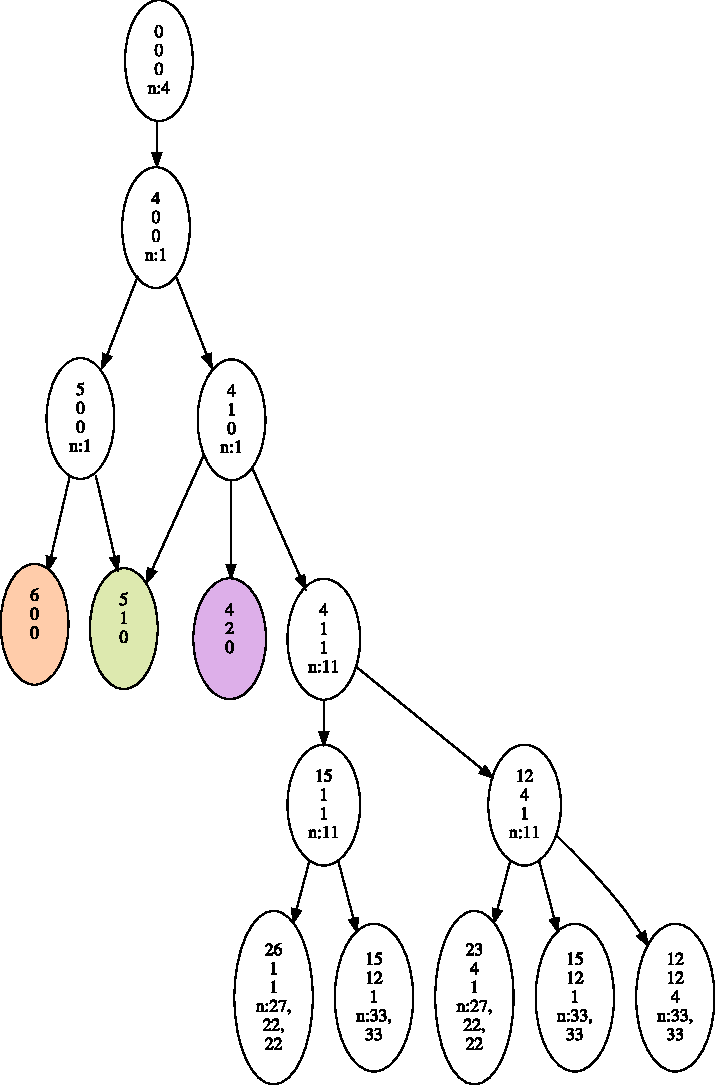
\includegraphics[scale=0.65]{img/big_picture.pdf}
  \caption{The beginning moves of the $45/33$ lower bound, scaled so
      that $T = 33$ and $S = 45$. The vertices contain the current
      loads of all three bins, and a string \texttt{n: $i$} with $i$
      being the next item presented by the \adversary. If there are
      several numbers after \texttt{n:}, the items are presented in
      the given order, regardless of packing by the player \algo. The coloured vertices are expanded in later figures.}
\end{figure}
\newpage
\begin{figure}
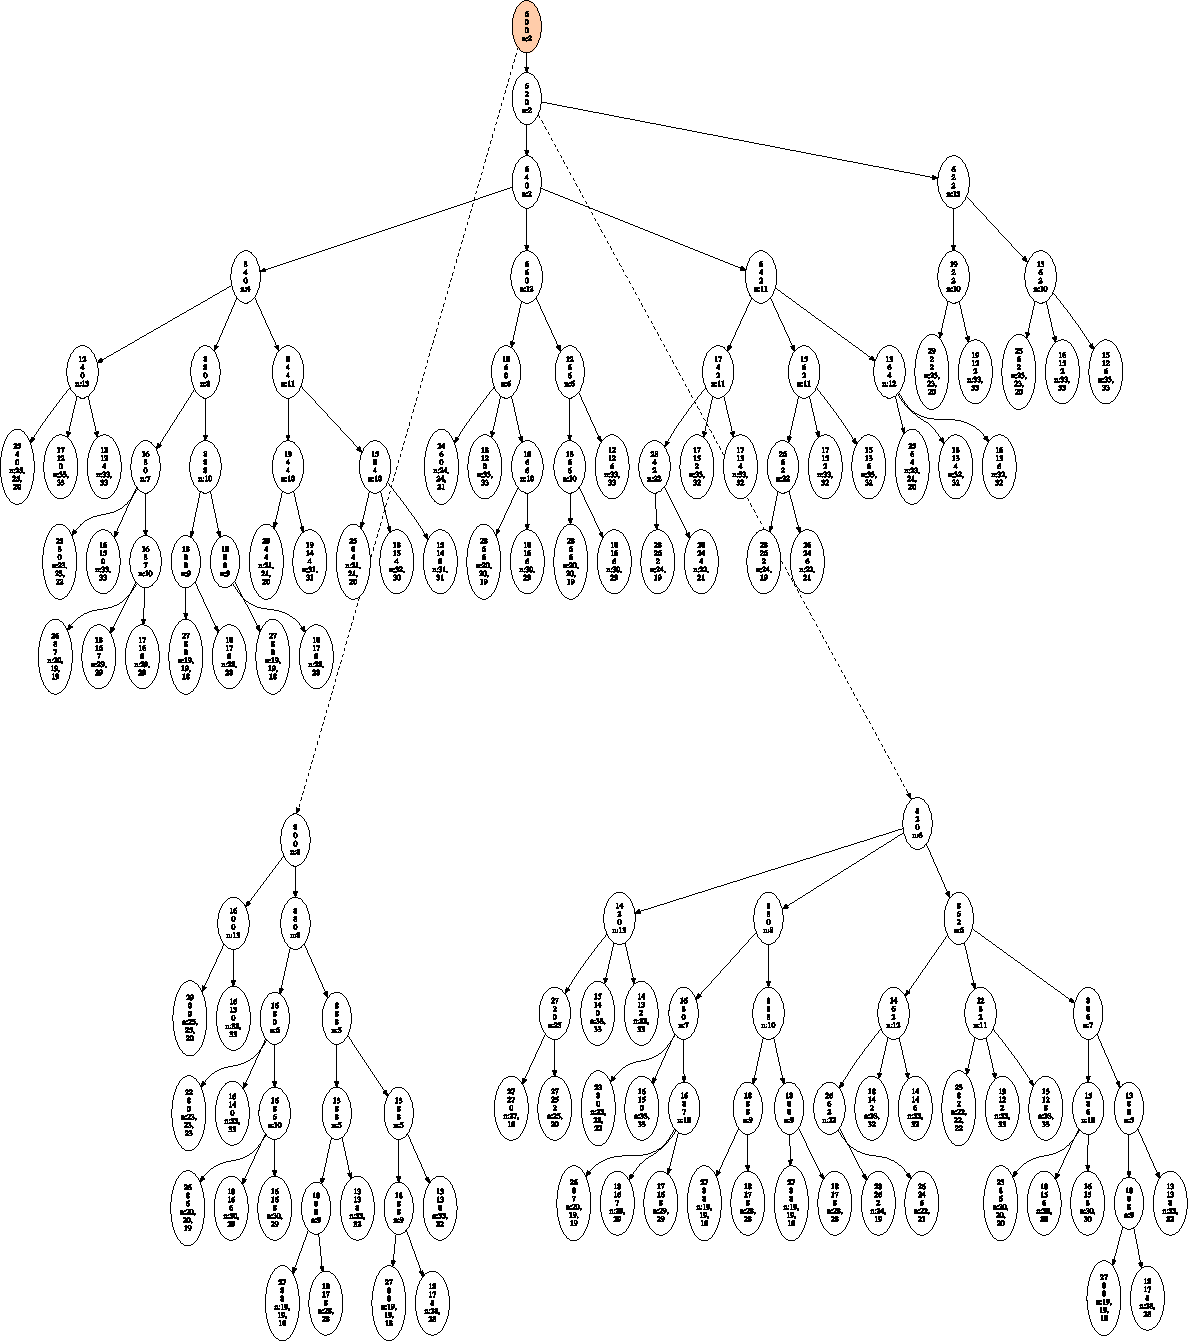
\includegraphics[scale=0.6]{img/6-0-0.pdf}
\caption{Game tree for the lower bound of $45/33$, starting with the bin configuration $(6,0,0,\{4,1,1\})$.}
\end{figure}

\begin{figure}
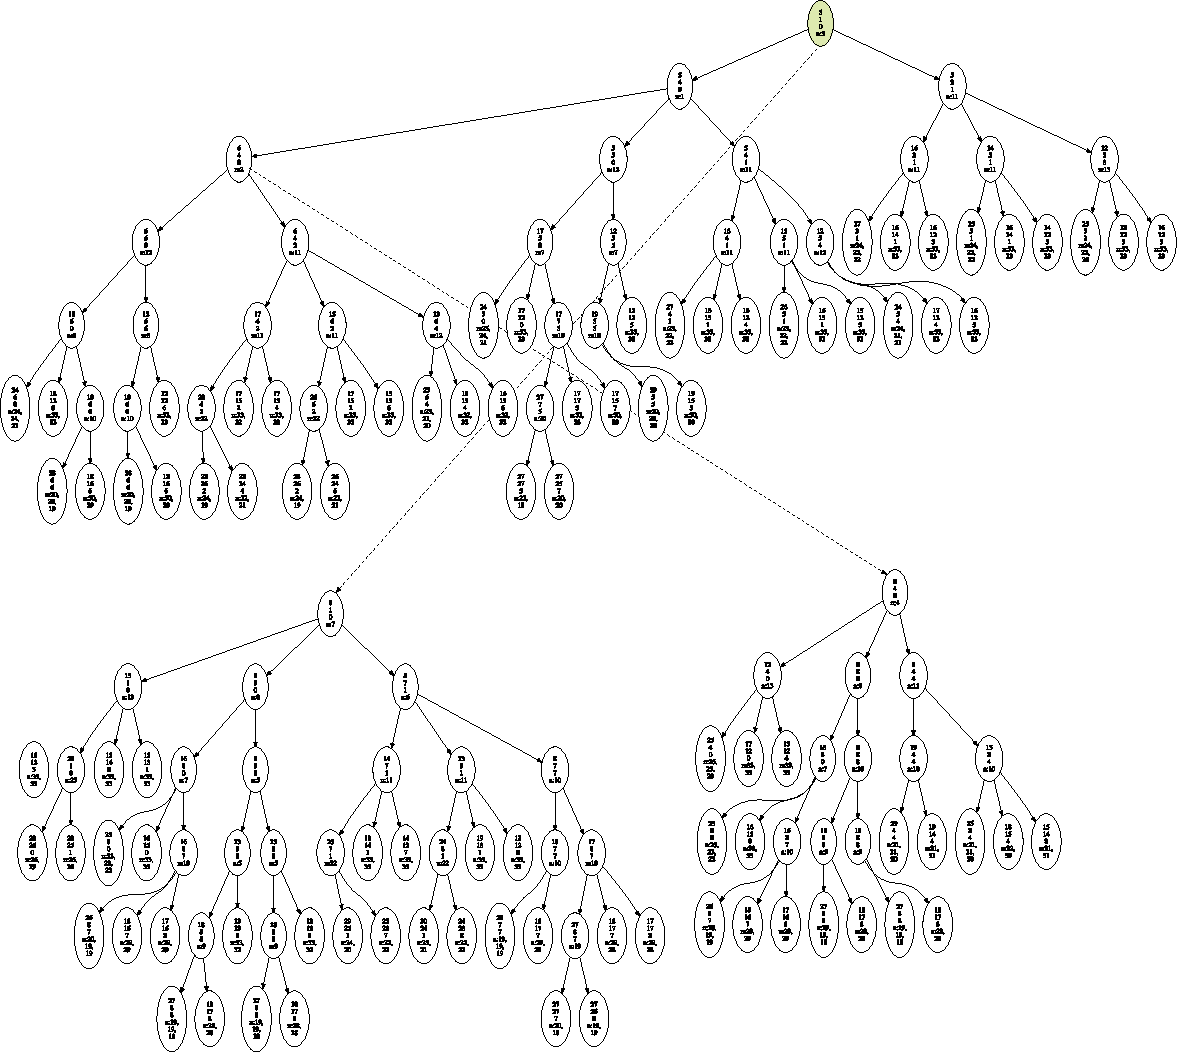
\includegraphics[scale=0.6]{img/5-1-0.pdf}
\caption{Game tree for the lower bound of $45/33$, starting with the bin configuration $(5,1,0,\{4,1,1\})$.}
\end{figure}

\begin{figure}
  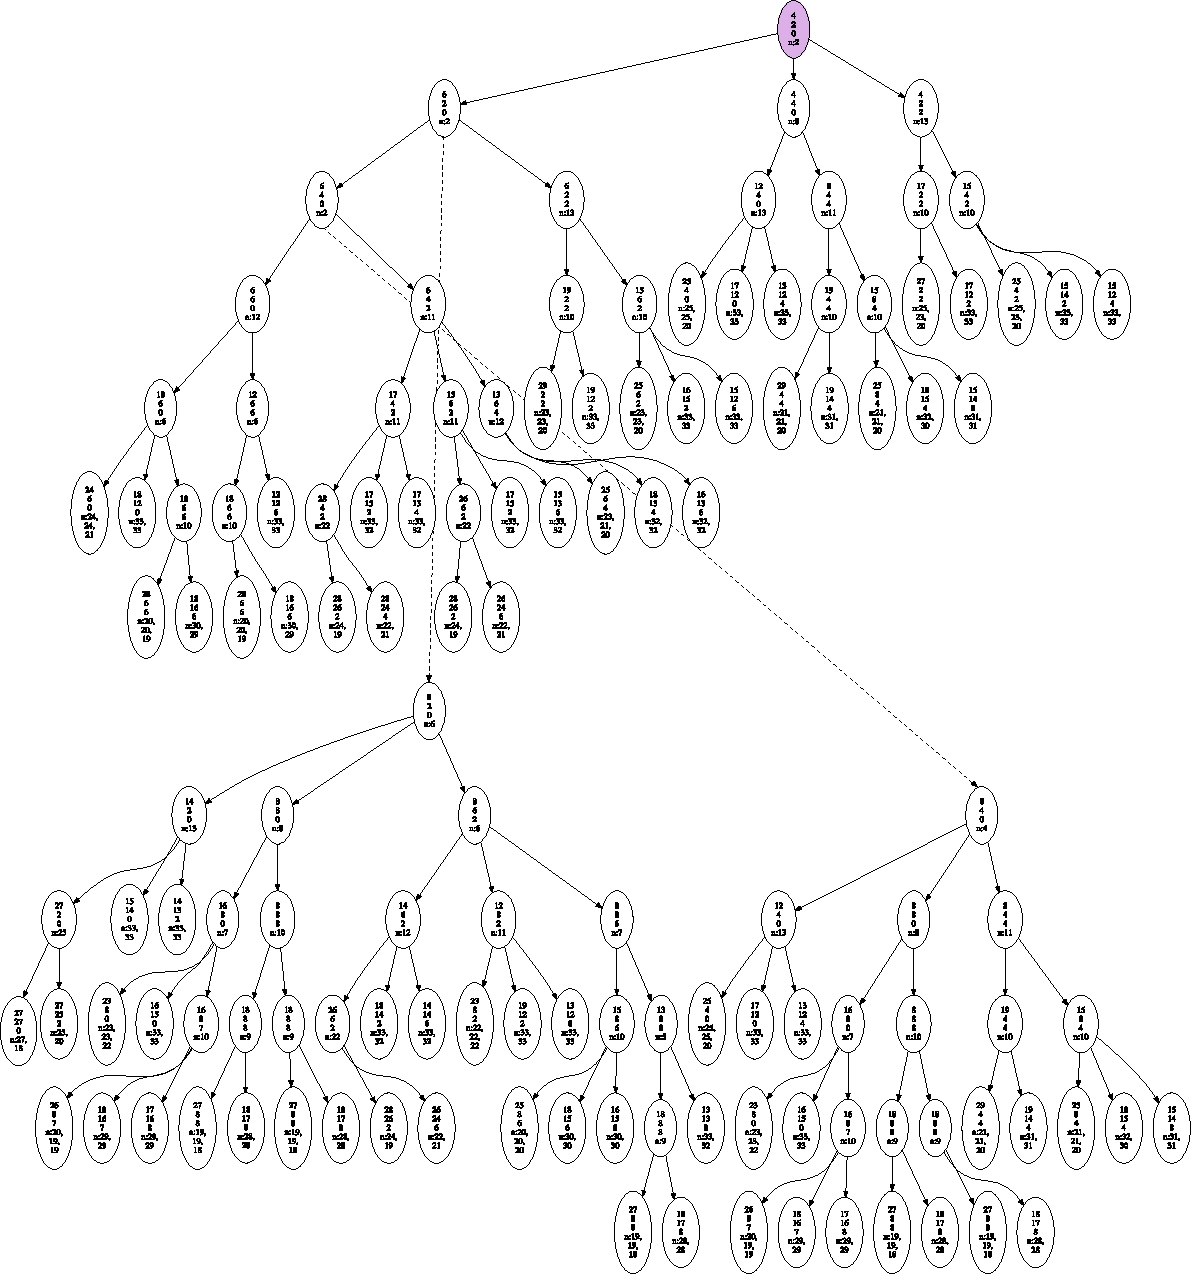
\includegraphics[scale=0.6]{img/4-2-0.pdf}
  \caption{Game tree for the lower bound of $45/33$, starting with the bin configuration $(4,2,0,\{4,1,1\})$.}
\end{figure}

\section{Verification of the results}\label{sec:verification}

\todo{Rewrite this.}

We give a compact representation of our game tree for the lower bound
of $45/33$ for $m=3$, which can be found in Appendix
\ref{sec:appendix}. The fully expanded representation, as given by our
algorithm, is a tree on 11053 vertices.

%TODO: exact number of vertices
For our lower bounds of $19/14$ for $m=4$ and $m=5$, the sheer size of
the tree (e.g. 4665 vertices for a compact representation for $m = 5$) prevents us from
presenting the game tree in its entirety.

We include the lower bound along with the implementations, publishing
it online at
\url{https://github.com/bohm/binstretch/}.

We have implemented a simple independent C++ program which verifies
that a given game tree is valid and accurate. While verifying our
lower bound manually may be laborious, verifying the correctness of
the C++ program should be manageable. The verifier is available along
with the rest of the programs and data.